\documentclass{beamer}
\usetheme{Madrid}
\colorlet{beamer@blendedblue}{green!40!black}
\setbeamertemplate{caption}[numbered]
\usepackage{amssymb, amsmath, amsthm}
\usepackage{physics, siunitx}
\usepackage{float, subcaption, graphicx}
\usepackage{hyperref}

\title{Chapter 2 - Plasma Physics}
\author{Hunt Feng\inst{1}}
\institute[Usask]
{
	\inst{1}%
	Faculty of Physics And Engineering Physics\\
	University of Saskatchewan
}
\date{\today}

%%%%%%%%%%%%%%%%%%%%
% section page 
%%%%%%%%%%%%%%%%%%%%
\AtBeginSection[]
{
	\begin{frame}{Outline of Presentation}
		\tableofcontents[currentsection]
	\end{frame}
}

\begin{document}
%%%%%%%%%%%%%%%%%%%%
% title and TOC
%%%%%%%%%%%%%%%%%%%%
\maketitle
\begin{frame}{Outline of Presentation}
	\tableofcontents
\end{frame}

%%%%%%%%%%%%%%%%%%%%
% contents 
%%%%%%%%%%%%%%%%%%%%
\section{Plasma Properties}
\begin{frame}{Tokamak Plasma}
    The typical plasma in tokamak has the following properties:
    \begin{figure}
        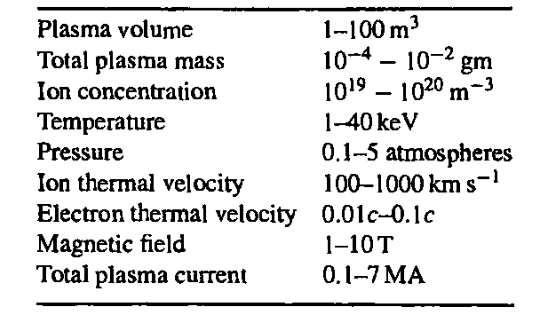
\includegraphics[width=0.7\textwidth]{figures/tokamak-plasma.png}
        \caption{Typical tokamak plasmas}
        \label{fig:typical-tokamak-plasmas}
    \end{figure}
\end{frame}

\begin{frame}{Debye Shielding}
    Due to the high mobility of electrons, the electric field from heavy ions will be shielded by electron cloud. The electric field is very small at certain distance away from ions. Hence, the plasma is quasineutral.

    The number density of ion and electron obey the Boltzmann distribution,
    \begin{equation}
        n_j = n_0 \exp(-\frac{e_j\phi}{T})
        \label{eq:boltzmann-distribution}
    \end{equation}
    The electric potential from an ion shielded by electrons is given by,
    \begin{equation}
        \phi = \frac{e}{4\pi\epsilon_0r} \exp(-\frac{\sqrt{2}r}{\lambda_D})
        \label{eq:electric-potential}
    \end{equation}
    where $\lambda_D$ is the Debye length and is defined by
    \begin{equation}
        \lambda_D = \left(\frac{\epsilon_0 T}{ne^2}\right)^2 = 2.35\times10^5\left(\frac{T}{n}\right)^2
        \label{eq:bebye-length}
    \end{equation}
\end{frame}

\begin{frame}{Plasma Frequency}
    If we pin ions as a static and uniform background, and perturb electrons, then electrons will oscillate around the static ions. The oscillation frequency is called electron plasma frequency, and is
    \begin{equation}
        \omega_{pe} = \left(\frac{ne^2}{\epsilon_0m_e}\right)^{1/2}
        \label{eq:electron-plasma-frequency}
    \end{equation}
    Similarly, the ion plasma has its oscillation frequency as well,
    \begin{equation}
        \omega_{pi} = \left(\frac{ne_i^2}{\epsilon_0m_i}\right)^{1/2}
        \label{eq:electron-plasma-frequency}
    \end{equation}
    where $e_i$ is the charge of ion.
\end{frame}
\section{Single Particle Motion}
\begin{frame}{Larmor Orbit}
    A charged particle gyrates in the plane that is perpendicular to the magnetic field lines. Its gyration radius is called Larmor radius,
    \begin{equation}
        \rho = \frac{mv_\perp}{eB}
        \label{eq:larmor-radius}
    \end{equation}
    where $v_\perp$ is the speed in the direction perpendicular to magnetic field B.

    The gyration frequency is called Larmor frequency or cyclotron frequency
    \begin{equation}
        \omega_c = \frac{eB}{m}
        \label{eq:cyclotron-frequency}
    \end{equation}
\end{frame}

\begin{frame}{Particle Motion along B}
    \begin{itemize}
        \item If B field is uniform and no E field along $\mathbf{B}$, then the particle is moving with constant velocity in the direction of $\mathbf{B}$.
        \item If B field is uniform and there is a non-zero component of E along $\mathbf{B}$, then the particle will experience a force $eE_\parallel$ along $\mathbf{B}$.
        \item If B field has gradient in the direction of $\mathbf{B}$ (assuming no E). Then the particle will experience a force $-\frac{\frac{1}{2}mv\perp^2}{B}\grad_\parallel B$.
    \end{itemize}
\end{frame}

\begin{frame}{Particle Drifts - $\mathbf{E\times B}$ Drift}
    \begin{equation}
        \mathbf{v}_{E\times B} = \frac{\mathbf{E\times B}}{B^2}
        \label{eq:e-cross-b-drift}
    \end{equation}
    \begin{figure}
        \centering
        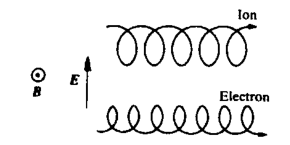
\includegraphics[width=0.7\textwidth]{figures/e-cross-b-drift.png}
        \caption{$\mathbf{E\times B}$ drift of ion and electron. $v_d=E/B$.}
        \label{fig:e-cross-b-drift}
    \end{figure}
\end{frame}

\begin{frame}{Particle Drifts - $\grad B$ Drift}
    \begin{equation}
        \mathbf{v}_{\grad B} = \text{sign}(e)\frac{1}{2}\rho\frac{\mathbf{B}\times\grad B}{B^2}v_\perp
        \label{eq:grad-b-drift}
    \end{equation}
    where $\text{sign}(e)$ is the sign of particle charge.
    \begin{figure}
        \centering
        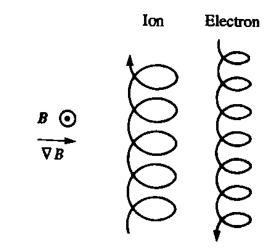
\includegraphics[width=0.4\textwidth]{figures/grad-b-drift.png}
        \caption{A gradient of B perpendicular to B gives ion and electron drifts in opposite directions.}
        \label{fig:grad-b-drift}
    \end{figure}
\end{frame}

\begin{frame}{Particle Drifts - Curvature Drift}
    \begin{equation}
        \mathbf{v}_{\grad B} = \frac{v_\parallel^2 + \frac{1}{2}v_\perp^2}{\omega_c}\frac{\mathbf{B}\times\grad B}{B^2}
        \label{eq:curvature-drift}
    \end{equation}
    \begin{figure}
        \centering
        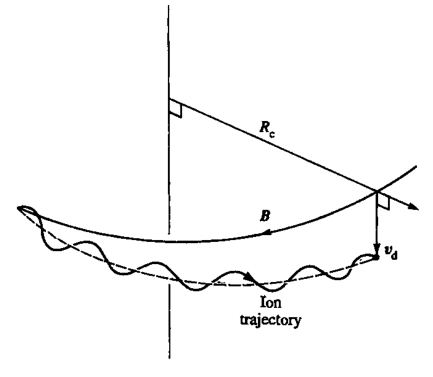
\includegraphics[width=0.5\textwidth]{figures/curvature-drift.png}
        \caption{Ion drift due to magnetic field curvature. Electrons drift in the opposite directions.}
        \label{fig:}
    \end{figure}
\end{frame}

\begin{frame}{Particle Drifts - Polarization Drift}
    \begin{equation}
        \mathbf{v}_{\grad B} = \frac{1}{\omega_cB}\dv{\mathbf{E}}{t}
        \label{eq:polarization-drift}
    \end{equation}
    \begin{figure}
        \centering
        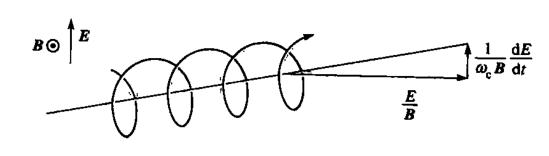
\includegraphics[width=0.7\textwidth]{figures/polarization-drift.png}
        \caption{Polarization drift of an ion caused by an increasing electric field perpendicular to the magnetic field. The electron drifts is in the opposite direction.}
        \label{fig:polarization-drift}
    \end{figure}
\end{frame}

\begin{frame}{Adiabatic Invariants}
    \begin{itemize}
        \item First adiabatic invariant: The magnetic moment, $\mu = \frac{\frac{1}{2}mv_\perp^2}{B}$, is constant if $\mathbf{B}$ changes very slowly.
        \item Second adiabatic invariant: This invariant $J$ is constant when the particle has a larger scale periodic motion. And $J = \oint v_\parallel\dd{l}$ where $\dd{l} = \mathbf{b}\cdot\dd{\mathbf{x}}$, $\mathbf{b}$ is the unit vector along $\mathbf{B}$.
        \item Third adiabatic invariant: If the periodic motion involved $J$ is subject to a drift and results in a larger scale periodic motion, then $J_3=\int v_d\dd{l}$ is invariant.
    \end{itemize}
\end{frame}
\section{Kinetic Theory}
\begin{frame}{Fokker-Planck Equation}
    \begin{equation}
        \dv{f}{t} + \mathbf{v}\cdot\pdv{f}{\mathbf{x}} + \frac{e}{m}(\mathbf{E+v\times B})\cdot\mathbf{v}\cdot\pdv{f}{\mathbf{v}} = \left(\pdv{f}{t}\right)_c
        \label{eq:fokker-planck-equation}
    \end{equation}

    In collisionless plasma, $(\partial_tf)_c=0$. The collisionless Fokker-Planck equation has another name called Vlasov equation.
\end{frame}

\begin{frame}{Landau Damping}
    \begin{itemize}
        \item Landau damping is predicted by kinetic theory.
        \item Damping exists for waves even in collisionless plasma as well.
        \item The damping comes from the interaction of wave with particles travelling at the phase velocity, $\omega/k$.
    \end{itemize}
    If we perturb the Vlasov equation, with $f = f_0 + f_1$ and $E = E_0 + E_1$, where the subscript 1 indicates that it is a perturbation quantity, we will have dispersion relation
    \begin{equation}
        \omega = \omega_p(1+3k^2\lambda_D^2)^{1/2} - i\left(\frac{\pi}{8}\right)^{1/2}\frac{\omega_p}{(k\lambda_D)^3}\exp\left[-\frac{1}{2}\left(\frac{1}{k^2\lambda_D^2}+3\right)\right]
        \label{eq:landau-damping}
    \end{equation}
\end{frame}

\begin{frame}{Collision}
    \begin{equation}
        \left(\pdv{f}{t}\right)_c = - \sum_\alpha\pdv{v_\alpha}(\expval{\Delta v_\alpha} f) + \frac{1}{2}\sum_{\alpha,\beta}\pdv[2]{}{v_\alpha}{v_\beta}\,(\expval{\Delta v_\alpha\Delta v_\beta}f)
        \label{eq:fokker-planck-collision-term}
    \end{equation}
    where $\expval{\Delta v_\alpha}$ is coefficient of dynamic friction and $\expval{\Delta v_\alpha\Delta v_\beta}$ diffusion tensor, and they are defined as
    \begin{align}
        \expval{\Delta v_\alpha}               & = \int \psi\Delta v_\alpha\dd{\Delta\mathbf{v}}/\Delta t \label{eq:coefficient-of-dynamic-friction} \\
        \expval{\Delta v_\alpha\Delta v_\beta} & = \int \psi\Delta v_\alpha\Delta v_\beta\dd{\Delta\mathbf{v}}/\Delta t \label{eq:diffusion-tensor}
    \end{align}
    The $\psi(\mathbf{v},\Delta\mathbf{v})$ is the probability of a particle with velocity $\mathbf{v}$ being scattered by $\Delta\mathbf{v}$ in the time $\Delta t$.
\end{frame}

\begin{frame}{Gyro-averaged Kinetic Equations}
    If the plasma phenomenon involves processes which are slow compared to the Larmor frequency and which vary slowly in space compared to the Larmor radius of the individual particle, then we can average the particle motion over the fast Larmor motion,
    \begin{equation}
        \dv{\bar{f}}{t} + \mathbf{v}_g\cdot\pdv{\bar{f}}{\mathbf{x}} + \left(e\mathbf{E}\cdot\mathbf{v}_g+\mu\pdv{B}{t}\right)\pdv{\bar{f}}{K} = \left(\pdv{\bar{f}}{t}\right)_c
        \label{eq:gyro-averaged-equation}
    \end{equation}
    where $\mu=mv_\perp^2/2B$ is the magnetic moment, $K=\frac{1}{2}mv^2$ is the kinetic energy, and
    \begin{equation}
        \mathbf{v}_g = v_\parallel\mathbf{b} + \frac{\mathbf{E\times B}}{B^2} + \frac{v_\parallel^2\mathbf{b\times (b\cdot\grad)b} + \mu\mathbf{b\times\grad}B}{\omega_c}
        \label{eq:guiding-center-velocity}
    \end{equation}
    is the guiding center velocity, and $\mathbf{b}=\mathbf{B}/B$ and $\omega_c = eB/m$.

    \begin{itemize}
        \item Gyro-averaged equation reduces 1 dimension compare to the Fokker-Planck equation.
        \item Not valid if the equilibrium possesses magnetic shear.
    \end{itemize}
\end{frame}

\begin{frame}{Fokker-Planck Equation for a Plasma}
    We first define the so-called Rosenbluth potentials,
    \begin{equation}
        \begin{aligned}
            H_j(\mathbf{v}) & = \left(1+\frac{m}{m_j}\right)\int \frac{f_j(\mathbf{v})}{\abs{\mathbf{v-v_j}}}\dd{\mathbf{v_j}} \\
            G_j(\mathbf{v}) & = \int f_j(\mathbf{v})\abs{\mathbf{v-v_j}}\dd{\mathbf{v_j}}
        \end{aligned}
        \label{eq:rosenbluth-potentials}
    \end{equation}
    The collision term, Eq.(\ref{eq:fokker-planck-collision-term}), can be written using these potentials,
    \begin{equation}
        \begin{aligned}
            \left(\pdv{f}{t}\right)_c = \sum_j \frac{e^2Z^2Z_j^2\ln\Lambda}{4\pi\epsilon_0^2m^2}
             & \left[ -\pdv{v_\alpha}\left(\pdv{H_j(\mathbf{v})}{v_\alpha} f(\mathbf{v})\right)\right.                                         \\
             & \left. +\frac{1}{2}\pdv[2]{}{v_\alpha}{v_\beta}\,\left(\pdv[2]{G_j(\mathbf{v})}{v_\alpha}{v_\beta} f(\mathbf{v})\right) \right]
        \end{aligned}
        \label{eq:collision-term-rosenbluth}
    \end{equation}
    Notice that $\expval{\Delta v_\alpha}$ and $\expval{\Delta v_\alpha\Delta v_\beta}$ can also be expressed using Rosenbluth potentials.
\end{frame}

\begin{frame}{Fokker-Planck Equation for a Plasma - Continued}
    We can also write the collision term as symmetric Landau integral form,
    \begin{equation}
        \left(\pdv{f}{t}\right)_c = \sum_j \frac{e^2Z^2Z_j^2\ln\Lambda}{4\pi\epsilon_0^2m^2} \pdv{v_\alpha}
        \int \left(  \frac{f_j(\mathbf{v_j})}{m} \pdv{f(\mathbf{v})}{v_\beta} - \frac{f(\mathbf{v})}{m_j} \pdv{f_j(\mathbf{v_j})}{v_{j\beta}} \right) u_{\alpha\beta} \dd{\mathbf{v_j}}
        \label{eq:collision-term-landau-integral}
    \end{equation}
    where $\mathbf{u=v-v_j}, u_{\alpha\beta}=(u^2\delta_{\alpha\beta} - u_\alpha u_\beta)/u^3$.

    In this way, once we have the initial distributions of each species, we can numerically solve the Fokker-Planck equation, Eq.(\ref{eq:fokker-planck-equation}).
\end{frame}

\begin{frame}{Fokker-Planck Coefficient under Maxwellian Distribution}
    Under Maxwellian distribution, we can calculate Rosenbluth potentials, Eq.(\ref{eq:rosenbluth-potentials}). The collision term $(\partial_t f)_c$, Eq.(\ref{eq:collision-term-rosenbluth}), becomes
    \begin{equation}
        \left(\pdv{f}{t}\right)_c = -\grad_v\cdot[\expval{\Delta\mathbf{v}_\parallel}f - \grad_\parallel(D_\parallel f) - D_\perp\grad_\perp f]
        \label{eq:collision-term-form}
    \end{equation}
    where $\grad_v$ means the divergence in velocity space, and the diffusion coefficients are
    \begin{align}
        D_\parallel & = \frac{1}{2}\expval{(\Delta v_\parallel)^2}                                                     \\
        D_\perp     & = \frac{1}{2}\expval{(\Delta v_{\perp\alpha})^2} = \frac{1}{2}\expval{(\Delta v_{\perp\beta})^2}
    \end{align}
\end{frame}

\begin{frame}{Relaxation Processes}
    The heat exchange time, $\tau_{ij}$, is defined by
    \begin{equation}
        \dv{T_i}{t} = \frac{T_j - T_i}{\tau_{ij}}
        \label{eq:heat-exchange-time-definition}
    \end{equation}
    For electrons and single charged ions the heat exhange time is
    \begin{equation}
        \tau_{ie} = \tau_{ei} = \frac{m_i}{2m_e}\tau_e
        \label{eq:heat-exchange-time-electron-ion}
    \end{equation}
    where $\tau_e$ is the electron collision frequency
    \begin{equation}
        \tau_e = 3(2\pi)^{3/2}\frac{\epsilon_0^2m_e^{1/2}T_e^{3/2}}{ne^4\ln\Lambda}
        \label{eq:electron-collision-frequency}
    \end{equation}
\end{frame}

\begin{frame}{Collision Times}
    If the temperature is in unit \unit{\kilo\eV}, then collision times (in \unit{\s}) are
    \begin{align}
        \tau_e & = 1.09\times10^{16}\frac{T_e^{3/2}}{n_iZ^2\ln\Lambda}                \\
        \tau_i & = 6.60\times10^{17}\frac{(m_i/m_p)^{1/2}T_i^{3/2}}{n_iZ^2\ln\Lambda}
    \end{align}
    Fig.

    The Coulomb logarithm is defined as $\ln\Lambda = \int_0^{\lambda_D} \frac{r\dd{r}}{r_0^2+r^2}$.
    \begin{itemize}
        \item electron-electron collisions
              \[ \ln\Lambda = 14.9-\frac{1}{2}\ln(n_e/10^20) + \ln T_e, \;\; \text{$T_e$ in \unit{\kilo\eV}} \]
        \item electron-ion collisions ($T\gtrsim 10$\unit{\eV})
              \[ \ln\Lambda = 15.2-\frac{1}{2}\ln(n_e/10^20) + \ln T_e, \;\; \text{$T_e$ in \unit{\kilo\eV}} \]
    \end{itemize}
\end{frame}

\begin{frame}{Collision Times - Figure}
    \begin{figure}
        \centering
        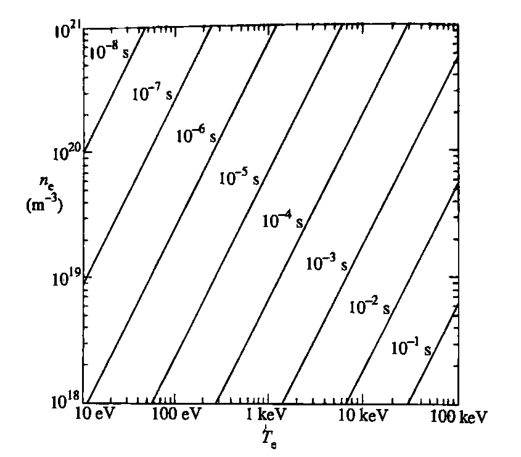
\includegraphics[width=0.6\textwidth]{figures/collision-time.png}
        \caption{Values of $\tau_e$ plotted against electron density and electron temperature.}
        \label{fig:collision-time}
    \end{figure}
\end{frame}

\begin{frame}{Resistivity}
    Resistivity can be defined by Ohm's law, $E=\eta j$.
    \begin{itemize}
        \item Singly charged ions (good for $B=0$ or in $B_\parallel$ direction):
              \begin{equation}
                  \eta_s = 0.51\frac{m_e^{1/2}e^2\ln\lambda}{3\epsilon_0^2(2\pi T_e)^{3/2}}, \;\;\;\text{$T_e$ in \unit{\kilo\eV}}
                  \label{eq:resistivity-singly-charged-ion}
              \end{equation}
        \item Plasma composed of several ion species,
              \[ \eta = Z_{eff}\eta_s, \;\; Z_{eff} = \frac{\sum_j n_jZ_j^2}{\sum_j n_jZ_j} \]
              It is obvious that $Z_{eff}=1$ for hydrogen plasma.
    \end{itemize}
    Worth to mention, resistivity in $B_\perp$ direction is almost twice of that in $B_\parallel$ direction,
    \[ \eta_\perp = \frac{m_e}{n_ee^2\tau_e} = 1.96\eta_\parallel \]
\end{frame}

\begin{frame}{Runaway Electrons - Simple Estimate}
    \begin{figure}
        \centering
        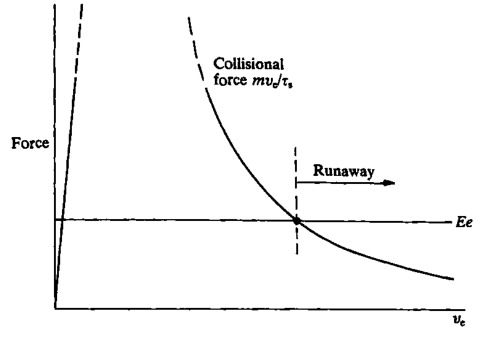
\includegraphics[width=0.5\textwidth]{figures/runaway-electrons.png}
        \caption{The electric field force, $Ee$, and the collisional force for an electron with a velocity $v_e$.}
        \label{fig:runaway-electrons}
    \end{figure}
    Fig.\ref{fig:runaway-electrons} shows that, electrons in the tail of velocity distribution might run away due to the presence of electric field. The critical velocity is
    \begin{equation}
        v_c^2 = \frac{3ne^3\ln\Lambda}{4\pi\epsilon_0^2m_eE} = 2.3\times10^{-4}\frac{n}{E}\; \unit{\m\tothe{2}\per\s\tothe{2}}, \;\; \ln\Lambda=17
        \label{eq:critical-velocity}
    \end{equation}
\end{frame}

\section{Fluid Theory}
\begin{frame}{Fluid Equations - Moments of $f$}
    From the distribution function $f(\mathbf{x},\mathbf{v}',t)$, we can get its moments by multiplying it with functions of $\mathbf{v}'$ and integrate them.
    \begin{equation}
        \begin{aligned}
            n          & = \int f(\mathbf{x},\mathbf{v}',t)\dd{\mathbf{v}'}                                \\
            \mathbf{v} & = \frac{1}{n}\int f(\mathbf{x},\mathbf{v}',t)\mathbf{v}'\dd{\mathbf{v}'}          \\
            \mathbf{P} & = m\int f(\mathbf{x},\mathbf{v}',t)(\mathbf{v'-v})(\mathbf{v'-v})\dd{\mathbf{v}'}
        \end{aligned}
        \label{eq:distribution-moments}
    \end{equation}
    where $\mathbf{P}$ is pressure tensor. For spatial homogeneous distribution function, the scalar pressure is given by
    \begin{equation}
        p = \frac{1}{3}m\int f(\mathbf{x},\mathbf{v}',t)(\mathbf{v'-v})^2\dd{\mathbf{v}'}
        \label{eq:scalar-pressure}
    \end{equation}
\end{frame}

\begin{frame}{Fluid Equations - Equations of Motion}
    Apply the same procedure in previous slide to Fokker-Planck Equation, Eq.(\ref{eq:fokker-planck-equation}), we are able to get equations of motions,
    \begin{itemize}
        \item Continuity Equation:
              \begin{equation}
                  \pdv{n}{t} + \div(n\mathbf{v}) = 0
                  \label{eq:conservation-of-density}
              \end{equation}
        \item Momentum Equation:
              \begin{equation}
                  nm\left( \pdv{\mathbf{v}}{t} + \mathbf{v}\cdot\grad\mathbf{v} \right) = -\div\mathbf{P} + nZe(\mathbf{E+v\times B}) + \mathbf{R}
                  \label{eq:conservation-of-momentum}
              \end{equation}
              where $\mathbf{R} = \int m\mathbf{v'}\left(\pdv{f}{t}\right)_c\dd{\mathbf{v'}}$.
    \end{itemize}
    We can continue this process and get more equations of higher moments $f$, e.g. heat equation.

    Fluid equations are only valid when the mean free path is small enough compare to the macroscopic scale. So not valid for high temperature plasma.
\end{frame}

\begin{frame}{Magnetohydrodynamics - Ideal MHD}
    To close the set of fluid equations, we need an extra equation of state (EOS), the adiabatic equation,
    \begin{equation}
        \dv{t}\,(p\rho^{-\gamma}) = 0
        \label{eq:adibatic-equation}
    \end{equation}

    Using the vacuum Maxwell's equations, and fluid equations together with EOS, we have the so-called ideal MHD equations,
    \begin{table}
        \centering
        \caption{The equations of ideal mhd.}
        \begin{tabular}{ll}
            \hline
            $\pdv{\rho}{t}           = -\rho\div\mathbf{v}           $ & $\mu_0\mathbf{j} = \curl\mathbf{B}$           \\
            $\rho\dv{\mathbf{v}}{t}  = \mathbf{j\times B} - \grad{p} $ & $\pdv{\mathbf{B}}{t}     = - \curl\mathbf{E}$ \\
            $\dv{p}{t}               = -\gamma p\div\mathbf{v}       $ & $\mathbf{E + v\times B}  = 0$                 \\
            \hline
        \end{tabular}
        \label{table:ideal-mhd}
    \end{table}
\end{frame}

\begin{frame}{Magnetohydrodynamics - Resistive MHD}
    To get resistive MHD equations, we only need to replace the adiabatic equation to
    \begin{equation}
        \dv{t}\,\left(\frac{p}{\gamma-1}\right) = \frac{\gamma}{\gamma-1}p\div\mathbf{v} + \eta j^2
        \label{eq:resistive-adibatic-equation}
    \end{equation}

    And the $\mathbf{E+v\times B} = 0$ to Ohm's law $\mathbf{E+v\times B} = \eta\mathbf{j}$
\end{frame}

\begin{frame}{Plasma Diamagnetism}
    \begin{itemize}
        \item Plasma is always diamagnetic due to the Larmor motions of particles weakens the applied magnetic field, see.
        \item The total diamagnetic current is given by $\mathbf{j = j_s + j_d}$, where $\mathbf{j_s} = \mathbf{b}\times\grad(p/B)$ is the current induced by particle gyration, and $\mathbf{j_d} = \mathbf{b}\times (p/B^2)\grad B$ is the drift current.
    \end{itemize}
\end{frame}

\begin{frame}{Plasma Diamagnetism - Figures}
    \begin{figure}
        \begin{subfigure}[b]{0.4\textwidth}
            \centering
            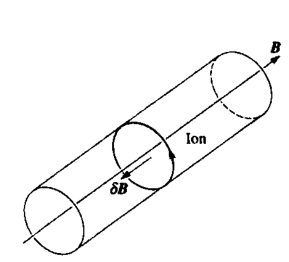
\includegraphics[width=0.7\textwidth]{figures/plasma-diamagnetism.png}
            \caption{Ions with a given velocity having Larmor orbits on a cylinder produce a magnetic field $\delta B$ inside the cylinder, this field being in the opposite direction to the total magnetic field B.}
            \label{fig:plasma-diamagnetism}
        \end{subfigure}%
        \begin{subfigure}[b]{0.4\textwidth}
            \centering
            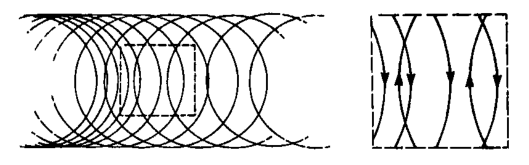
\includegraphics[width=\textwidth]{figures/diamagnetic-current.png}
            \caption{Showing how a density gradient of stationary orbits give rise to a current. The current arises through a local imbalance of upward and downward moving particles as illustrated in the enlarged secion.}
            \label{fig:diamagnetic-current}
        \end{subfigure}
    \end{figure}
\end{frame}

\begin{frame}{Braginskii Equations}
    \begin{itemize}
        \item Coulomb collisions do not change the number of particles.
        \item Friction force: $\mathbf{R_u} = - (m_en/\tau_e)(0.51u_\parallel + u_\perp) = ne(\eta_\parallel j_\parallel + \eta_\perp j_\perp)$, where $\mathbf{u=v_e-v_i}$
        \item Thermal force: $\mathbf{R_T} = -0.71n\grad_\parallel T_e - \frac{3}{2}\frac{n}{\abs{\omega_{ce}\tau_e}\mathbf{b}\times\grad T_e}$
        \item Ion heating: $Q_i = \frac{3m_e}{m_i}\frac{n}{\tau_e}(T_e-T_i)$.
        \item Electron heating: $Q_e = -\mathbf{R\cdot u} - Q_i = \eta_\parallel j_\parallel^2 + \eta_\perp j_\perp^2 + \frac{1}{ne}\mathbf{j\cdot R_T} + \frac{3m_e}{m_i}\frac{n}{\tau_e}(T_i-T_e)$
    \end{itemize}
    Some interesting things,
    \begin{itemize}
        \item The ratio of parallel to perpendicular thermal conductivity is $(\omega_{c}\tau)^2$. It is $10^{13}$ for electrons and $10^{16}$ for ions.
        \item In parallel direction, electron thermal conductivity is larger than that of ions by a factor $\sim (m_i/m_e)^2$ because of their long collision time.
        \item In perpendicular direction, the relationship is reversed because of the larger ion Larmor radius.
        \item The ohm heating $\eta j^2$ appears only in electrons because they only transfer $\sim m_e/m_i$ of energy to ions.
    \end{itemize}
\end{frame}

\begin{frame}{Plasma Waves - Dispersion Relations}
    \begin{itemize}
        \item Transverse EM wave:
              \begin{equation}
                  \omega^2 = k^2c^2 + \omega_p^2
                  \label{eq:transverse-wave}
              \end{equation}
        \item Sound wave:
              \begin{equation}
                  \omega^2 = k^2c_s^2,\;\; c_s^2 = \gamma\frac{p_i + p_e}{nm_i}
                  \label{eq:}
              \end{equation}
        \item Shear Alfven wave, see Fig:
              \begin{equation}
                  \omega = k_xv_A,\;\; v_A = B_0/\sqrt{\mu_0\rho}
                  \label{eq:shear-alfven-wave}
              \end{equation}
        \item Magnetosonic waves:
              \begin{equation}
                  \frac{\omega^2}{k^2} = \frac{1}{2} \{ c_s^2 + v_A^2 \pm [(c_s^2+v_A^2)^2 - 4c_s^2v_A^2\cos^2\theta]^{1/2} \}
                  \label{eq:magnetosonic-wave}
              \end{equation}
              The fast magnetosonic wave given by choosing the $+$ sign, and the slow magnetosonic wave given by choosing the $-$ sign.
    \end{itemize}
\end{frame}

\begin{frame}{Plasma Wave - Alfven Wave}
    \begin{figure}
        \centering
        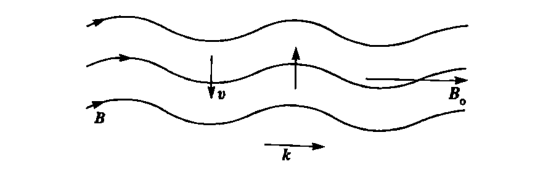
\includegraphics[width=0.6\textwidth]{figures/simple-alfven-wave.png}
        \caption{Simple Alfven wave with $k\parallel B_0$. The fluid velocity oscillates in the plane of the figure.}
        \label{fig:simple-alfven-wave}
    \end{figure}
    \begin{figure}
        \centering
        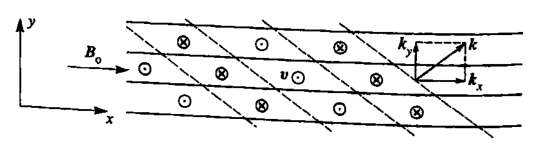
\includegraphics[width=0.6\textwidth]{figures/shear-alfven-wave.png}
        \caption{General shear Alfven wave. $B_0$ and $k$ lie in the plane of the figure and the velocity oscillation is perpendicular to this plane. The wave propagates along $x$ with the Alfven velocity $v_A$.}
        \label{fig:shear-alfven-wave}
    \end{figure}
\end{frame}

\begin{frame}{Plasma Wave - Magnetosonic Wave}
    \begin{figure}
        \centering
        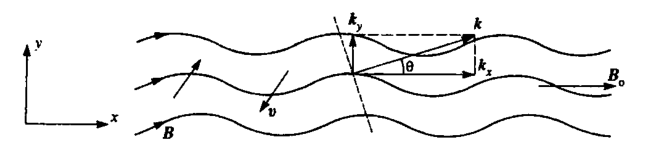
\includegraphics[width=0.7\textwidth]{figures/magnetosonic-wave.png}
        \caption{The magnetosonic wave has velocity oscillations in the plane containing $B_0$ and $k$.}
        \label{fig:magnetosonic-wave}
    \end{figure}
    \begin{figure}
        \centering
        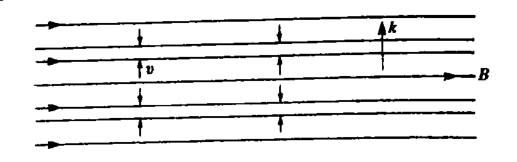
\includegraphics[width=0.6\textwidth]{figures/magnetosonic-wave-fast.png}
        \caption{The fast magnetosonic with $k\perp B_0$. The oscillations involve compression of both the fluid and the magnetic field.}
        \label{fig:magnetosonic-wave-fast}
    \end{figure}
\end{frame}

%%%%%%%%%%%%%%%%%%%%
% references
%%%%%%%%%%%%%%%%%%%%
\newpage
\begin{frame}[allowframebreaks]
	\bibliographystyle{abbrv}
	\bibliography{../references}
	\nocite{*}
\end{frame}

\end{document}
